\section{Biologische Grundlagen}
\label{biologie}
\thispagestyle{plain}

Das visuelle System geh"ort zu den am gr"undlichsten untersuchten
Sinnessystemen der Gro"shirnrinde.  Das liegt nur zum einen an der gut
zug"anglichen Lage der Cortexareale, die f"ur die erste visuelle
Reizverarbeitung zust"andig sind.  Sie befinden sich bei S"augern direkt
unterhalb der Sch"adeldecke im hinteren Pol des Gro"shirns.  Zum anderen
kann man das visuelle System einfach und unter kontrollierten,
reproduzierbaren Bedingungen "uber die Augen reizen. Es ist sozusagen das
``Wasserstoff--Atom der Hirnforschung''; theoretische Konzepte und
Erkl"arungsmodelle lassen sich im Experiment am visuellen System
falsifizieren, bzw. k"onnen im Wechselspiel mit dem Experiment verfeinert
werden.

In den folgenden Abschnitten werden die f"ur das weitere Verst"andnis der
Arbeit ben"otigten biologischen Zusammenh"ange, sowie die in dieser Arbeit
behandelten Ph"anomene erl"autert. Der letzte Abschnitt dieses Kapitels
geht dabei auf Ergebnisse einer Datenanalyse ein, bei der in Zusammenarbeit
mit Siegrid L"owel vom Max--Planck--Institut f"ur Hirnforschung die
geometrische Beziehung zwischen Okulardominanz-- und Orientierungskarten
aus A17 schielender Katzen untersucht wurde.

\subsection{Skizze des visuellen Systems von S"augern}

\subsubsection{Die Sehbahn}
\label{sehbahnkap}

Die Netzhaut (Retina) ist eine, aus drei verschiedenen Zelltypen
bestehende, schichtartig aufgebaute Struktur, welche die Umwandlung
physikalischer Lichtreize in neuronale Signale vornimmt.  Der schichtartige
Aufbau ist dabei charakteristisch f"ur viele andere Strukturen im
Zentralnervensystem. Durch einfallendes Licht wird zun"achst eine beim
Menschen aus ca. 125~Millionen Photorezeptoren (St"abchen und Zapfen)
bestehende Zellschicht stimuliert.  Die visuelle Information wird dann in
einer zwischengelagerten Zellschicht und in einer Schicht aus
ca. 1~Millionen Ganglienzellen weiterverarbeitet. Die Nervenendungen
(Axone) der Ganglienzellen b"undeln sich an der Papille und verlassen das
Auge als Sehnerv. Schon aus diesem anatomischen Verh"altnis von 125:1 wird
deutlich, da"s in der Retina eine Vorverarbeitung visueller Information
stattfinden mu"s (vgl. Abschn.~\ref{rf}).  Die Sehnerven aus beiden Augen
verzweigen sich im \emph{Chiasma opticum}: hier wechselt etwa die H"alfte
aller Sehnervfasern die Hemisph"are, w"ahrend der Rest ungekreuzt
weiterverl"auft (siehe Abb.~\ref{sehbahn}).  Alle Nervenfasern, die aus den
jeweils linken Netzhauth"alften entstammen, werden so in die linke
Hirnh"alfte weitergeleitet (analog bei der rechten Netzhauth"alfte).  Auf
diese Weise ist hinter dem Chiasma opticum die rechte Gesichtsfeldh"alfte
in der linken Hemisph"are und die linke in der rechten Hemisph"are
repr"asentiert.  Nur ein kleiner Bereich des zentralen Gesichtsfeldes ist
beidseitig vertreten.

In jeder Hemisph"are projiziert nun ein Teil des neuzusammengesetzten
Nervenfaserb"undels (\emph{Tractus opticus}) auf den seitlichen Knieh"ocker
(\emph{Corpus geniculatum laterale}, LGN) im Thalamus.  Die geb"undelten
Fasern aus den Netzh"auten werden hier in geordneter Weise wieder
aufgef"achert und m"unden in mehreren Zellschichten, die wie in einem
Sandwich "ubereinander liegen.  Einzelne Knieh"ockerzellen erhalten nur
Eing"ange von einem Auge: Eine Zelle im LGN ist entweder ``links"augig''
oder ``rechts"augig''.  Diese beiden Zellsorten liegen getrennt voneinander
in verschiedenen Schichten.

\begin{figure}[t]
\begin{center}
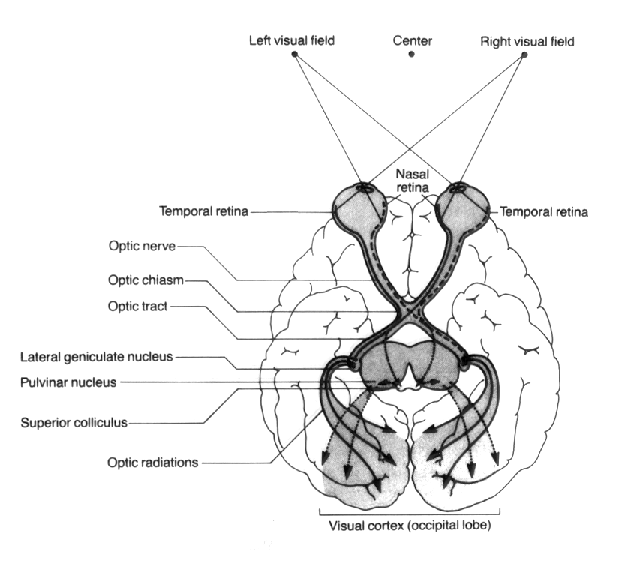
\epsfig{file=pics/sehbahn.eps,width=12cm}
\end{center}
\caption{Skizze der Sehbahn im menschlichen Gehirn von den Augen bis zum
prim"aren visuellen Cortex \protect\citeaffixed{churchland:1992}{aus}.}
\label{sehbahn}
\end{figure}

Am Ende des LGN treten Nervenfasern aus allen Schichten zu einem breiten
Band zusammen, der \emph{Radiatio optica}, das zur Sehrinde aufsteigt.  Die
Sehrinde ist in mehrere abgegrenzete Gebiete, sogenannte \emph{Areale}
unterteilt, die zum Teil sehr spezifische Leistungen (wie z.B.
Bewegungs--, Form-- und Farbsehen) erbringen und in zahlreichen Kan"alen
untereinander Information austauschen.  Das au"senweltn"achste,
\emph{prim"are} visuelle Areal (in Affen V1, in Katzen h"aufig A17 genannt)
ist --- wie die Retina und das LGN --- schichtartig strukturiert.  Im Affen
projiziert das LGN ausschlie"slich zum prim"aren visuellen Cortex, in
Katzen auch in umliegende Areale.  Auch bei der Projektion vom LGN in den
prim"aren visuellen Cortex f"achern die Fasern wieder in geordneter Weise
auf: Die Topologie der Abbildung vom Gesichtsfeld in den Cortex bleibt
somit erhalten.

\begin{figure}[t]
\begin{center}
\begin{minipage}[m]{5cm}
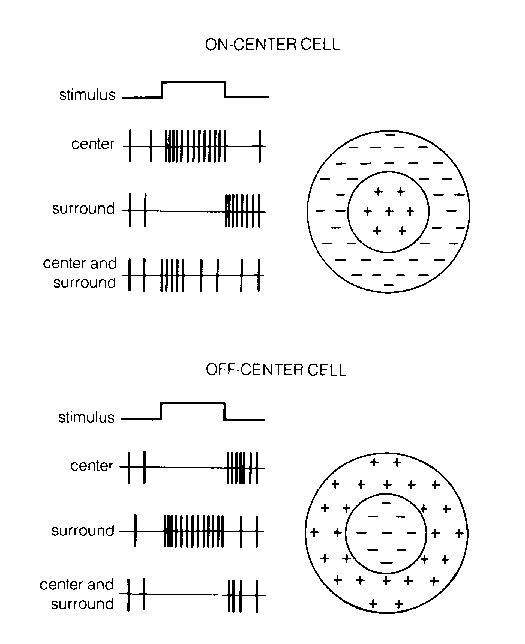
\epsfig{file=pics/rf_onoff.eps,width=5cm}
\end{minipage}
\hskip1cm
\begin{minipage}[m]{6cm}
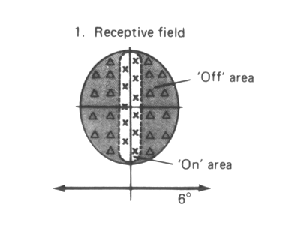
\epsfig{file=pics/rf_simple.eps,width=6cm}
\end{minipage}
\end{center}
\caption{\textbf{a)} Skizze der radialsymmetrischen rezeptiven Felder
sogenannter ``Zentrum--Umfeld--Zellen'' (rechts). Die mit~``$+$''
markierten Gebiete kennzeichnen Bereiche, in denen eine Stimulation zur
Erregung der Zelle f"uhrt (``Exzitation''); in den mit~``$-$'' markierten
Bereichen f"uhrt eine Stimulation zur Hemmung der Zelle
(``Inhibition''). Nach ihrem Antwortverhalten (skizziert in der linken
Spalte) unterscheidet man 2 Typen: \emph{ON--Zentrum}--Zellen und
\emph{OFF--Zentrum}--Zellen. \textbf{b)} Skizze eines rezeptiven Feldes
einer sog. ``einfachen Zelle''. Ein zentrales, schmales exzitatorisches
Gebiet ist von symmetrischen, inhibitorischen Gebieten umgeben. Der
optimale Stimulus f"ur diese Zelle ist ein vertikal orientierter
Lichtbalken (von $\approx1^\circ\times 8^\circ$ Gr"o"se) im Zentrum des
rezeptiven Feldes.}
\label{rfsimple}
\end{figure}

\subsubsection{Rezeptive Felder}
\label{rf}

Bei den Zellen im prim"aren visuellen Cortex stellt man --- wie auch bei
den Ganglienzellen der Retina und den Zellen im LGN --- eine
Spezialisierung auf gewisse Reizmerkmale fest.  Dabei bestimmen in der
Retina zun"achst wenige einfache Merkmale, wie z.B.  Position und Gr"o"se
eines Reizes, das Antwortverhalten einer Ganglienzelle (jede Zelle im
Zentralnervensystem hat eine Ruheaktivit"at, die bei geeigneter Stimulation
drastisch erh"oht werden kann).  Das Gebiet genau abgegrenzter Position und
Gr"osse auf der Sinnesoberfl"ache, welches bei Stimulation zur Aktivierung
einer Zelle f"uhrt --- also der Verantwortungsbereich dieser Zelle ---
bezeichnet man auch als das \emph{rezeptive Feld} dieser Zelle (siehe
Abb.~\ref{rfsimple}a).  Am Ende der Sehbahn reagieren die Zellen auf immer
abstraktere Merkmale der Au"senwelt.  So lassen sich die Zellen im
prim"aren visuellen Cortex oft nur noch mit Lichtreizen einer ganz
bestimmten Position, Gr"osse und Orientierung stimulieren (einfache Zellen,
siehe Abb.~\ref{rfsimple}b).  Eine andere Zellsubpopulation erh"oht ihre
Aktivit"at nur, wenn sich der Stimulus in einer bestimmten Richtung bewegt
(komplexe Zellen).  Zus"atzlich sind die Zellen hier spezialisiert auf
Stimuli aus einem bestimmten Auge (man nennt dies ``okulare Dominanz'' der
Zellen).

Etwas verallgemeinernd bezeichnet man oft auch die Menge aller Merkmale,
die ein Reiz besitzen mu"s, um die Aktivit"at einer bestimmten Zelle zu
maximieren, als das rezeptive Feld dieser Zelle.  Die Zunahme der
Spezialisierung ist Ausdruck der Konvergenz im visuellen System: entlang
der Sehban erhalten fast alle Zellen Eing"ange von mehr als einer anderen,
vorgelagerten Zelle. (Mit dieser anatomischen Beobachtung l"a"st sich
bereits die Pr"aferenz visueller corticaler Zellen f"ur bestimmte
Stimulusorientierungen erkl"aren; siehe Abb.~\ref{opmodel}.)

\begin{figure}[p]
\begin{center}
\epsfig{file=pics/opmodel.eps,width=9cm}
\end{center}
\caption{Einfaches Model der Orientierungspr"aferenz \protect\cite{hubel:1962}: 
Die Axone mehrerer Zentrum--Umfeld--Zellen konvergieren auf eine einfache
Zelle. Dadurch, da"s die rezeptiven Felder der Zentrum--Umfeld--Zellen auf
der Sinnesoberfl"ache entlang einer Linie angeordnet sind, antwortet die
einfache Zelle selektiv auf Lichtbalken einer bestimmten Orientierung.}
\label{opmodel}
\end{figure}

\begin{figure}[p]
\begin{center}
\begin{minipage}[m]{5.5cm}
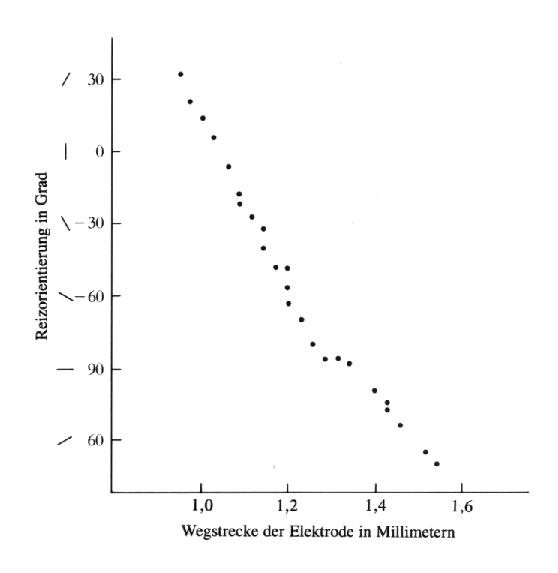
\epsfig{file=pics/opelektrode1.eps,width=5.5cm}
\end{minipage}
\hskip1cm
\begin{minipage}[m]{5.5cm}
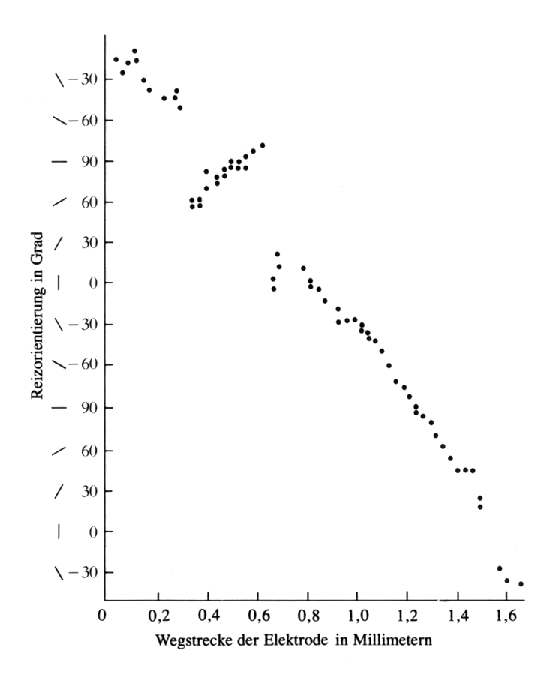
\epsfig{file=pics/opelektrode2.eps,width=5.5cm}
\end{minipage}
\end{center}
\caption{Ergebnis eines typischen Experiments mit tangentialer
Elektrodenf"uhrung durch Area 17 in einer Katze f"ur 2 verschiedene
Wegf"uhrungen, \protect\citeaffixed{hubel:1989}{aus}.  Aufgetragen ist
jeweils die pr"aferierte Reizorientierung der abgeleiteten Zelle gegen"uber
der Entfernung vom Ausgangspunkt der Messung.  \textbf{a)} Die bevorzugte
Reizorientierung "andert sich stetig und linear mit der Wegstrecke.
\textbf{b)} In dieser Messung "andert sich der Drehsinn zweimal sprunghaft
innerhalb einer Strecke von wenigen zehntel Millimetern.}
\label{opelektrode}
\end{figure}

\subsubsection{Kolumn"are Organisation der prim"aren Sehrinde}

Mit einer Mikroelektrode, die schrittweise durch den Cortex geschoben wird,
kann man experimentell den Verlauf der rezeptiven Feldeigenschaften von
Zellen entlang einer Linie im Cortex bestimmen
\citeaffixed{hubel:1989}{siehe z.B.}: Durch die  Mikroelektrode ist
das elektrische Potential einer einzelnen Zelle me"sbar.  Das
Aktionspotential einer Zelle im ``Ruhezustand'', also ohne geeignete
Stimulation, "uberschreitet dabei nur gelegentlich eine kritische Schwelle,
oberhalb der die Zelle einen elektrischen Puls aussendet (die Zelle
``feuert'').  Wird nun ein geeigneter Stimulus auf die Retina projiziert,
so k"onnen die Merkmale dieses Stimulus (wie z.B. Gr"o"se, Position, usw.)
solange variiert werden, bis die ``Feuerrate'' der betrachteten Zelle
maximiert wurde: das rezeptive Feld der Zelle wurde gefunden.  Auf diese
Weise k"onnen innerhalb eines Experiments die rezeptiven Felder mehrerer
Zellen bestimmt werden.

Ein Ergebnis solcher Messungen ist, da"s die rezeptiven Feldeigenschaften
untereinanderliegender Zellen identisch sind. Tangential zur
Cortexoberfl"ache variieren die rezeptiven Feldeigenschaften der Zellen
dagegen i.a. graduell und in gesetzm"a"siger Weise mit der Position der
Zellen auf der Cortexoberfl"ache (vgl. Abb.~\ref{opelektrode}).  Das
prim"are visuelle Areal ist somit wie die meisten anderen
sinnesverarbeitenden Bereiche der Hirnrinde \emph{kolumn"ar} organisiert,
d.h.  Zellen sind zu funktionalen Einheiten (``Kolumnen'') von wenigen
Zehntelmillimetern Durchmesser zusammengefa"st, die sich zylinderf"ormig
radial in den Cortex erstrecken.

\subsection{Neuronale Karten}

Obwohl die Verschaltung der Retina mit dem prim"aren visuellen Areal, wie
in Abschnitt~\ref{sehbahnkap} dargestellt, "uber mehrere
``Relaisstationen'' verl"auft, bleibt die Topologie der Sinnesoberfl"ache
unter der Abbildung in den Cortex erhalten, d.h.  benachbarte Neurone im
Cortex haben benachbarte Verantwortungsbereiche im Gesichtsfeld.  Die im
letzten Abschnitt beschriebenen Mikroelektroden--Experimente lie"sen schon
fr"uh erkennen, da"s es sich bei dieser Projektion um eine
zweidimensionale, oftmals stetige Merkmalsabbildung handelt.  Aufgrund der
Nachbarschaftserhaltung l"a"st sich eine solche Abbildung auch als
\emph{Karte} der Au"senwelt ansehen.  Unter einer \emph{neuronalen Karte}
versteht man eine (h"aufig in Ortskoordinaten) parametrisierte Darstellung
des Verlaufs einer rezeptiven Feldeigenschaft "uber ein Cortexareal.  Das
naheliegendste Beispiel einer neuronalen Karte ist die sogenannte
\emph{retinotope Karte} im prim"aren visuellen Areal, bei der benachbarte
Neurone auf Reize reagieren, die benachbart im Gesichtsfeld angeordnet sind
(und deshalb benachbart auf die Retina abgebildet werden; dies erkl"art das
Attribut ``retinotop'').

Im prim"aren visuellen Cortex sind i.a. auch Karten abstrakterer Merkmale der
\mbox{Au"senwelt} angelegt. Diese sind der retinotopen Karte "uberlagert. 
Ein genaueres Bild dieser Karten f"ur ein ausgedehntes Gebiet mit Hilfe von
Mikroelektroden--Experimenten zu erhalten hie"se jedoch ``eine
dreidimensionale Frage mit einer eindimensionalen Me"smethode'' zu
beantworten \cite{hubel:1989}.  Mittlerweile gibt es jedoch geeignete
Methoden zur Messung neuronaler Karten. In den folgenden beiden Abschnitten
werden daher die wichtigsten Typen visueller neuronaler Karten zusammen mit
gebr"auchlichen Methoden zu ihrer Messung vorgestellt.

\subsubsection{Okulardominanzkarten}
\label{odkarten}

\begin{figure}[t]
\begin{center}
\begin{minipage}[m]{3.9cm}
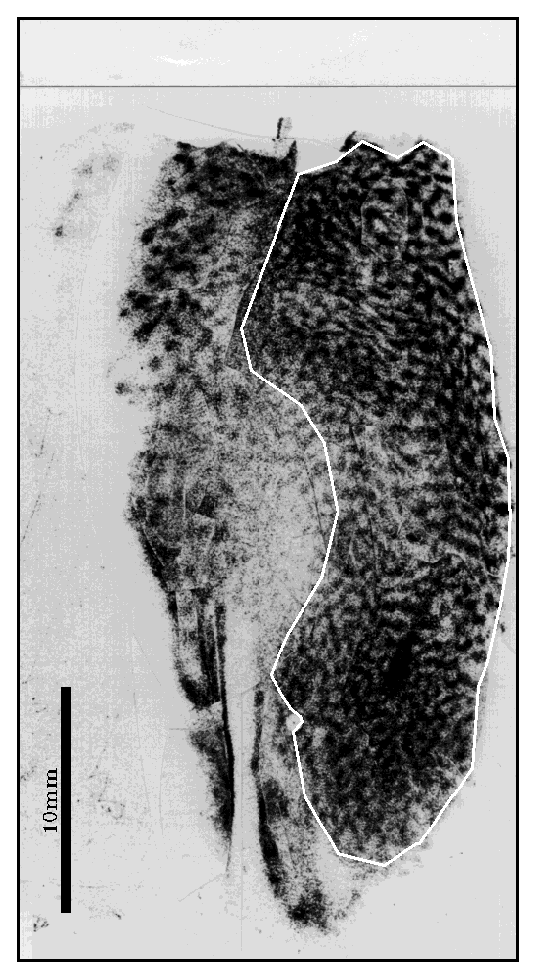
\epsfig{file=pics/normKatze.eps,width=3.9cm,clip=}
\end{minipage}
\hskip2cm
\begin{minipage}[m]{3.9cm}
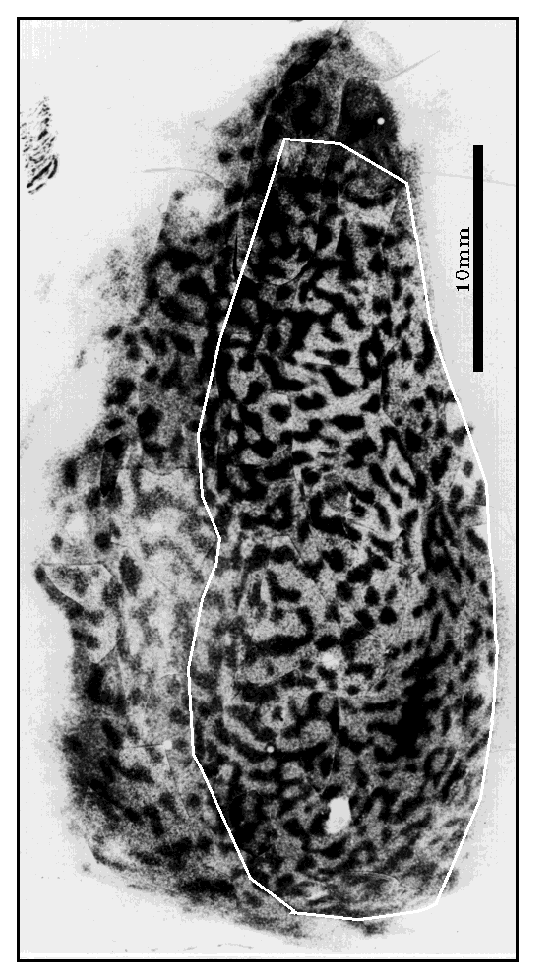
\epsfig{file=pics/strabKatze.eps,width=3.9cm}
\end{minipage}
\end{center}
\caption{Autoradiographie der Okulardominanzkarte aus A17 einer
normalsichtigen (links) und schielenden Katze (rechts)
\protect\citeaffixed{loewel:1987}{neurophysiologische Methode, Karten aus}.}
\label{odsiegrid}
\end{figure}

Neuroanatomische Verfahren zur Visualisierung einer
\emph{Okulardominanzkarte} beruhen auf radioaktiv markierten Stoffen
(typischerweise [$^3$H]--Prolin), die nach Injektion in ein Auge "uber
axonalen Transport von der Retina in den prim"aren visuellen Cortex
gelangen.  Auf diese Weise reichert sich der radioaktive Marker in den
Zellen an, die in Verbindung mit dem markierten Auge stehen.

Physiologische Messungen solcher Karten verwenden radioaktiv markierte
\mbox{2--deoxyglucose} (2DG), die dem Versuchstier intraven"os injiziert
wird. Danach wird ein Auge abgedeckt; der radioaktiv markierte Zucker
reichert sich nun in den Zellen an, die vom ge"offneten Auge getrieben
werden. Auf diese Art und Weise l"a"st sich die funktionale Struktur der
Okulardominanz sichtbar machen.

\setcounter{footnote}{1}
In beiden Experimenten werden anschlie"send d"unne Schnitte des Hirngewebes
angefertigt, die auf Glasplatten ausgefaltet und dann auf einen Film gelegt
werden. Nach langer Belichtung l"a"st sich anhand einer solchen
\emph{Autoradiographie} die Okularit"atskarte als Schw"arzungsverteilung
auf dem Film ablesen (siehe Abb.~\ref{odsiegrid}). Man erkennt eine
periodische Struktur, d.h. die schwarzen und wei"sen Gebiete (also die
Verantwortungsbereiche f"ur markiertes/unmarkiertes bzw. aktives/inaktives
Auge) wechseln sich in bestimmten, regelm"a"sigen Abst"anden ab.
Untersuchungen der Wellenl"ange\footnote{d.h. der "uber alle Richtungen
gemittelte Abstand, innerhalb dessen sich die Okulardominanz von einem Auge
zum anderen und wieder zur"uck ver"andert} von Okulardominanzkarten aus A17
normalsichtiger Katzen und A17 von Katzen, bei denen fr"uh ein
k"unstlicher, divergenter Schielwinkel der Augen induziert wurde
(\emph{Strabismus}), zeigen da"s die Wellenl"ange der
Okulardominanzstruktur bei schielenden Katzen gegen"uber der von
normalsichtigen Katzen systematisch erh"oht ist \cite{loewel:1994}.
\setcounter{footnote}{1}

\subsubsection{Orientierungskarten}

Zur Messung von \emph{Orientierungskarten} benutzt man heute die
sogenannten \emph{optical imaging}--Verfahren, die Mitte der achtziger
Jahre entwickelt wurden. Diese Verfahren nutzen die ver"anderten optischen
Eigenschaften aktiver Zellen und erm"oglichen dadurch die Sichtbarmachung
der funktionalen Anordung von Zellen unterhalb der Sch"adeldecke. Die
Ver"anderungen der optischen Eigenschaften k"onnen mit hochempfindlichen
Kameras durch die an einer Stelle ge"offnete Sch"adeldecke des
Versuchstiers abfotographiert werden.  Auf diese Weise erh"alt man Karten
f"ur beliebige, feste Stimulusmerkmale "uber ein ausgedehntes Gebiet von
einigen Millimetern Seitenl"ange.

Eine der Methoden bedient sich spannungsempfindlicher Farbstoffe, die auf
die Oberfl"ache des prim"aren visuellen Cortex aufgebracht werden. Das
Versuchstier sieht w"ahrend des Experiments auf einen Bildschirm, auf dem
z.B. horizontal orientierte Balken durchlaufen. Die Zellen, die am
deutlichsten auf diese Stimulation antworten, "au"sern dies durch ihre
erh"ohte elektrische Aktivit"at, welche wiederum die optischen
Eigenschaften des Farbstoffes ver"andert \cite{blasdel:1986,blasdel:1992a}.

Eine bessere Variante dieses Verfahrens ist durch Ausnutzung der
intrinsischen Signale der Cortexschicht nicht auf die langfristig
neurotoxischen, spannungsempfindlichen Farbstoffe angewiesen: Eine erh"ohte
Aktivit"at der Zellen zieht einen erh"ohten Blutdurchsatz in ihrer Umgebung
nach sich. Dieser erh"ohte Blutdurchsatz "au"sert sich wiederum in einer
erh"ohten Konzentration des Blutfarbstoffes H"amoglobin, der Licht der
Wellenl"ange $800nm$ absorbiert. Mit CCD--Kameras kann man die
Intensit"atsschwankungen auf der mit $800nm$--Licht beleuchteten
Cortexoberfl"ache aufnehmen. Die resultierende Hell/Dunkel--Verteilung
spiegelt die Inaktiv/Aktiv--Verteilung im beobachteten Gebiet wieder ---
also die neuronale Karte bez"uglich des au"sen anliegenden Stimulus
\cite{lieke:1989,grinvald:1991}.

Orientierungskarten f"ur eine feste Stimulusorientierung k"onnen auch mit
den in Abschnitt~\ref{odkarten} beschriebenen, neurophysiologischen
Methoden erhalten werden.  Der Vorteil des optischen Ableitens im Vergleich
zu neuroanatomischen oder neurophysiologischen Methoden liegt darin, da"s
man in solchen Experimenten die neuronalen Karten \emph{in vivo}
erh"alt. Insbesondere ist man so in der Lage, w"ahrend eines Experimentes
mehrere Karten f"ur verschiedene Stimulusbedingungen von einem Versuchstier
abzuleiten.

\begin{figure}[t]
\begin{center}
\begin{minipage}{10cm}
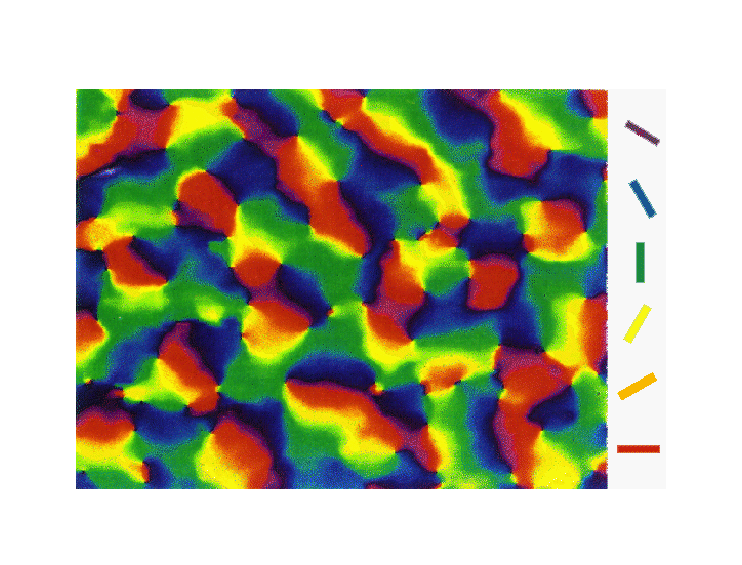
\epsfig{file=pics/OP_affe.eps,width=10cm}
\end{minipage}
\vskip0.5cm
\begin{minipage}[b]{4cm}
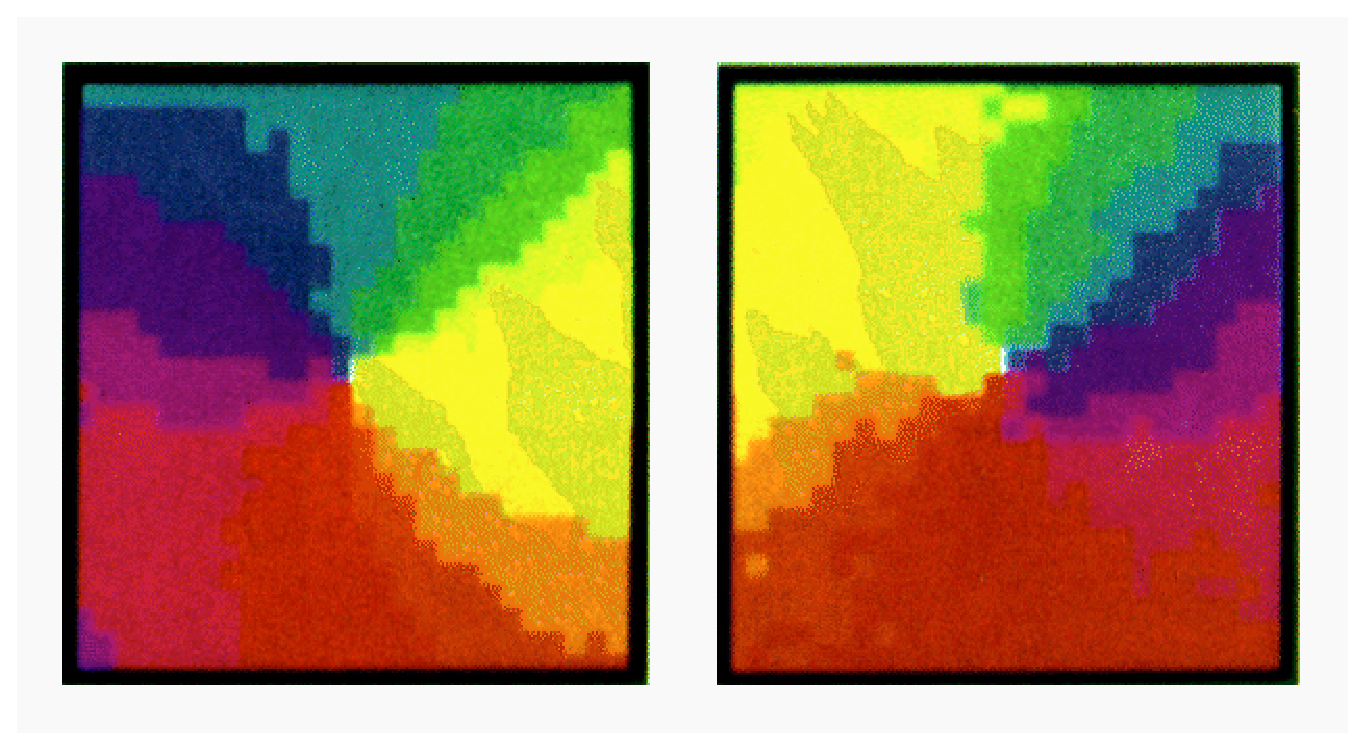
\epsfig{file=pics/pinwheels.eps,width=4cm}
\end{minipage}
\end{center}
\caption{\textbf{Oben:} Karte der Orientierungspr"aferenz aus dem prim"aren
visuellen Cortex eines Makaken \protect\citeaffixed{blasdel:1992b}{aus}.
\textbf{Unten:} Beispiel f"ur Pinwheels mit Chiralit"at~\eqref{chi}
$q_i=+\frac{1}{2}$ (links) und $q_i=-\frac{1}{2}$ (rechts). Die
Orientierung "andert sich beim linken Pinwheel im Uhrzeigersinn von gelb
nach rot (d.h. von rechts oblique nach horizontal); beim rechten Pinwheel
verl"auft die Orientierungs"anderung im Urzeigersinn von rot nach gelb
\protect\citeaffixed{bonhoeffer:1991}{d.h. von horizontal nach rechts
oblique; aus}.}
\label{opblasdel}
\end{figure}

Mehrere, in einem Versuch auf diese Art und Weise gemessenen
Aktivit"atsverteilungen (auch ``single--condition'' Karten genannt, siehe
z.B. Abb.~\ref{layout}, rechte Spalte) f"ur jeweils verschiedene
Orientierungen aus dem Intervall $[0^\circ,180^\circ)$ k"onnen dann
farblich codiert zu einer Orientierungskarte "uberlagert werden (siehe
Abb.~\ref{opblasdel}, oben).  Die Orientierungspr"aferenz als Funktion der
tangentialen Position $\mathbf{x}$ l"a"st sich folgenderma"sen formulieren:

\begin{equation*}
z(\mathbf{x})=\sum\limits_k A_k(\mathbf{x})\; \text{e}^{i2\theta_k}
\label{zfeld}
\end{equation*}

Alle zu den Stimulusorientierungen $\theta_k$ geh"orenden
Aktivit"atsverteilungen $A_k(\mathbf{x})$ werden hier zu einem komplexen
Feld~$z$ "uberlagert.  Aus diesem Feld ergibt sich die Orientierungskarte
durch die Relation

\begin{equation*}
\vartheta=\frac{1}{2}\text{arctan}(z).
\end{equation*}

Das auff"alligste Srukturelement einer solchen Orientierungskarte sind die
topologischen Punkt--Defekte, in deren Umgebung die
Iso--Orientierungsbereiche wie bei einem Windrad angeordnet sind (sie
werden daher oft auch als \emph{Pinwheels} berzeichnet): In einer
kreisf"ormigen Umgebung $C_i$ um eine Singularit"at "andert sich die
Orientierungspr"aferenz um $\pm 180^\circ$.  Die Positionen $\mathbf{x}_j$
dieser Singularit"aten sind dabei die Nullstellen des komplexen Feldes
$z(\mathbf{x})$. Man unterscheidet zwei Sorten solcher Punkt--Defekte nach
ihrer ``H"andigkeit'' (vgl. Abb.~\ref{opblasdel}, unten)

\begin{equation}
q_i=\frac{1}{2\pi}\oint_{C_i}\!\!\nabla\vartheta(\mathbf{x})\;ds = \pm
\frac{1}{2}
\label{chi}
\end{equation}

Beide Arten von Singularit"aten treten gleich h"aufig auf.  In allen
nat"urlichen Karten "andert sich die Orientierungspr"aferenz bei einem
vollem Umlauf um eine solche Singularit"at immer nur um $\pm 180^\circ$,
nicht aber um $\pm 360^\circ$ \citeaffixed{penrose:1979}{einen "Uberblick
"uber alle theoretisch m"oglichen Arten solcher Punktdefekte gibt}.

Das n"achst charakteristische Element einer Orientierungskarte sind die
sogenannten linearen Zonen. In diesen Gebieten, die etwa 50\% einer
Orientierungskarte ausmachen, laufen die Iso--Orientierungsbereiche
parallel "uber Strecken von bis zu $1mm$. Die Orientierung zwischen
benachbarten Iso--Orientierungsbereichen ver"andert sich stetig, d.h. ohne
Spr"unge (das Ergebnis eines Mikrolektrodenexperiments, bei dem die
Mikroelektrode senkrecht zur Richtung einer solchen linearen Zone bewegt
wurde, zeigt Abb.~\ref{opelektrode}a).

\subsection{Speziesunterschiede visueller Reizrepr"asentationen}
\label{unterschiede}

\begin{figure}[p]
\begin{center}
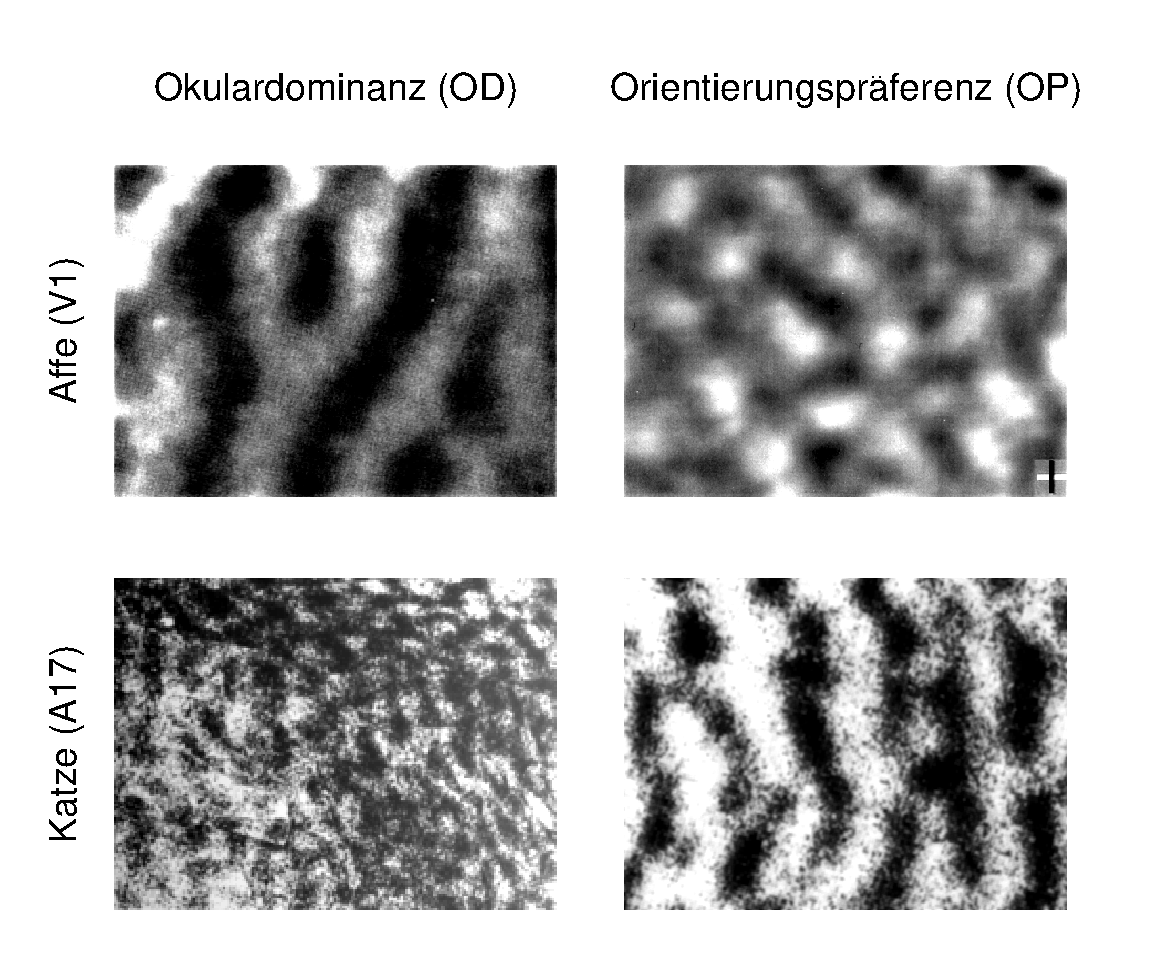
\epsfig{file=pics/monkeycat.eps,width=11cm}
\end{center}
\caption{Layoutvergleich kolumn"arer Strukturen aus dem prim"aren visuellen
Cortex von Katzen \protect\citeaffixed{loewel:1987,loewel:1990}{Daten aus} und Affen
\protect\citeaffixed{blasdel:1992a}{Daten aus}.}
\label{layout}
\end{figure}

\begin{figure}[p]
\begin{center}
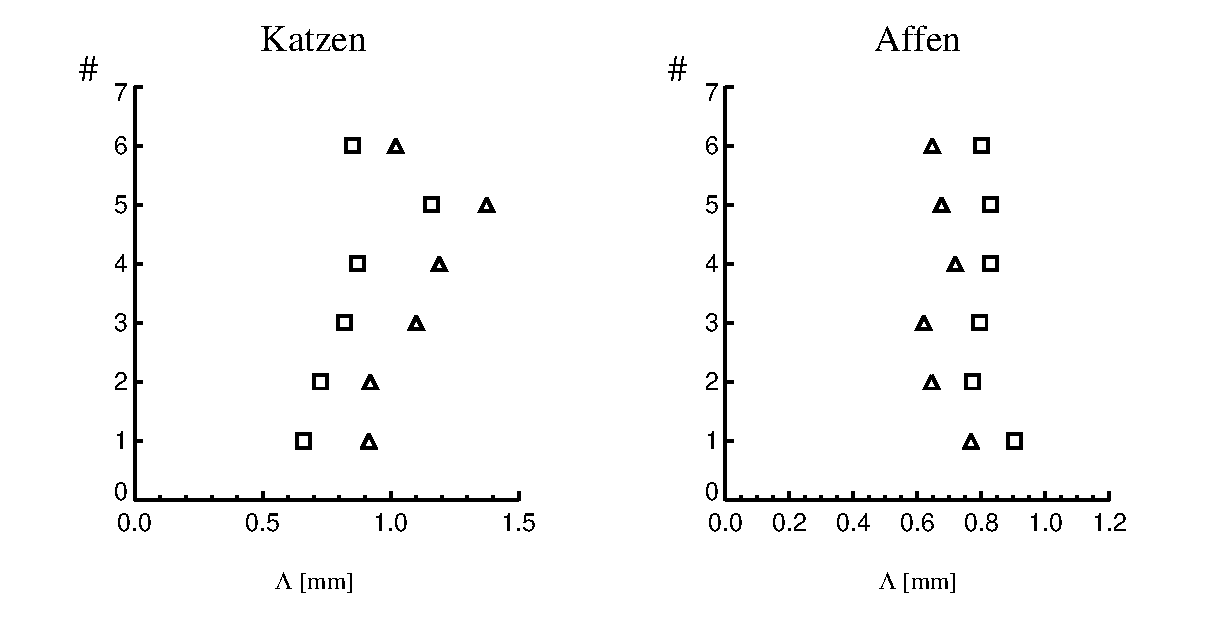
\epsfig{file=pics/wavelength.eps,width=10cm}
\end{center}
\caption{Wellenl"angenvergleich typischer Orientierungspr"aferenz-- und
Okulardominanzkarten aus dem prim"aren visuellen Cortex von Katzen und
Affen. Gezeigt ist das Verh"altnis der Wellenl"ange der
Orientierungspr"aferenz~($\triangle$) zur Wellenl"ange der
Okuardominanz~($\square$) f"ur mehrere Katzen
\protect\citeaffixed{loewel:1988}{links, Daten aus} und Affen
\protect\citeaffixed{oby:1993b}{rechts, Daten aus}.}
\label{wavelength}
\end{figure}

Vergleicht man nun neuronale Karten aus dem prim"aren visuellen Cortex von
Affen und Katzen, so erkennt man, da"s sich sowohl die
Orientierungspr"aferenz-- (OP) als auch Okulardominanzkarten (OD) in beiden
Spezies unterscheiden. Der erste, auff"alligste Unterschied betrifft das
Layout der jeweiligen Karten (siehe Abb~\ref{layout}): W"ahrend eine
typische Okulardominanzkarte aus V1 des Affen ein hochregul"ares Muster
paralleler B"ander aufzeigt, die senkrecht zu den Arealgrenzen verlaufen
und kaum verzweigen \cite{levayetal:1985,grinvald:1991}, besteht die
typische Okulardominanzkarte aus A17 der Katze aus einem Geflecht perliger,
aneinandergereihter Dom"anen ohne erkennbare Vorzugsrichtung
\cite{andersonetal:1988,loewel:1987}.  Eine ``single--condition''
Orientierungskarte dagegen, d.h. eine Karte, die f"ur einen Stimulus einer
bestimmten, festen Orientierung erhalten wurde, besteht im Affen aus
perligen, aneinandergereihten Dom"anen w"ahrend dieselbe Karte in der Katze
eine streifige Struktur paralleler B"ander aufzeigt.  Ber"ucksichtigt man
nur das Layout, so erscheint eine OD--Karte aus der Katze mit einer
OP--Karte aus dem Affen vergleichbar (und eine OP--Karte aus der Katze mit
einer OD--Karte aus dem Affen siehe dazu Abb.~\ref{layout}).

Ein weiterer Unterschied der Karten in beiden Spezies betrifft die
Wellenl"ange~$\Lambda$ der jeweiligen Strukturen
(vgl. Abb~\ref{wavelength}): Ein Vergleich der Wellenl"ange der
OD--Struktur mit der Wellenl"ange der OP--Struktur aus V1 des Affen ergibt,
da"s die mittlere Wellenl"ange der OD--Dom"anen immer gr"o"ser ist als die
der OP--Dom"anen.  Das Verh"altnis
$\Lambda_{\text{OD}}/\Lambda_{\text{OP}}$ ist ungef"ahr $6/5$
\cite{oby:1993b}. In der Katze verh"alt es sich genau umgekehrt: Hier ist
die mittlere Wellenl"ange der OP--Struktur immer gr"o"ser als die der
OD--Struktur; das Verh"altnis $\Lambda_{\text{OD}}/\Lambda_{\text{OP}}$
betr"agt ungef"ahr $4/5$ \cite{loewel:1988}.

Okulardominanzkarten aus dem prim"aren visuellen Cortex von Katzen und
Affen unterscheiden sich neben ihrer charakteristischen Wellenl"ange um ein
weiteres Merkmal: Der Grad der \emph{Okulardominanzsegregation} --- also
der Grad der Selektivit"at der Zellen f"ur eines der beiden Augen --- ist
im Affen sowie in der strabismischen und normalsichtigen Katze
unterschiedlich stark ausgepr"agt (siehe Abb.~\ref{okuhist}).

\begin{figure}[t]
\begin{center}
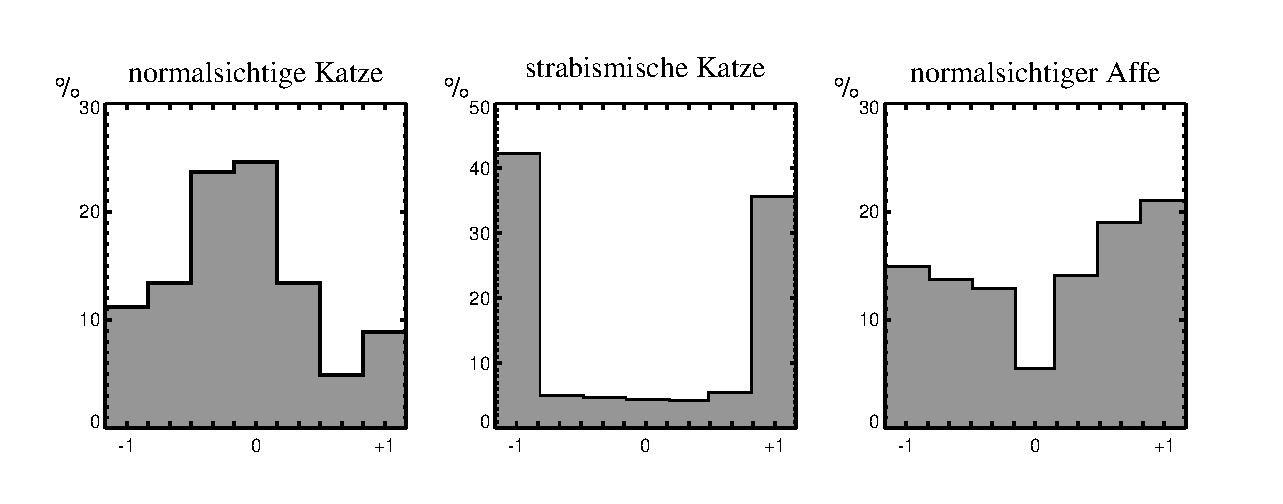
\epsfig{file=pics/okuhist.eps,width=\textwidth}
\end{center}
\caption{Okulardominanzhistogramme f"ur normalsichtige und strabismische
Katzen, sowie f"ur den Affen. Es ist die relative H"aufigkeit der Zellen,
die sich entweder nur vom linken ($-1$) oder nur vom rechten ($+1$) oder
von beiden Augen ($0$) stimulieren lassen aufgetragen. Bei normalsichtigen
Katzen sind die meisten Zellen binokular. Bei strabismischen Katzen und
beim Affen "uberwiegt die Zahl der Zellen, die sich auf eines der beiden
Augen spezialisiert hat \protect\citeaffixed{hubel:1989}{Daten aus}.}
\label{okuhist}
\end{figure}

\subsection[Geometrische Beziehung zwischen
Iso--Orientierungslinien$\ldots$]{Geometrische Beziehung zwischen
Iso--Orientierungslinien und Okulardominanz--Grenzlinien}
\label{90grad}

Untersuchungen von Okulardominanz-- und Orientierungskarten aus V1 des
Makaken ergaben, da"s es eine geometrische Beziehung zwischen den Grenzen
der Okulardominanzdom"anen und den Iso--Orientierungslinien gibt
\cite{bartfield:1992,oby:1993b}: In allen untersuchten F"allen zeigt die
Statistik ihrer Schnittwinkel einen Trend zu stumpfen Winkeln (siehe
z.B. Abb~\ref{odop_hist}, rechts).

F"ur die Katze liegt eine solche Untersuchung bislang noch nicht vor, da in
der normalsichtigen Katze der Grad der Okulardominanzsegregation zu schwach
ist, um optisches Ableiten der Okulardominanzkarte zu erlauben (die
Signalst"arke ist hier zu gering). Normalerweise wird die
Orientierungskarte in der Katze durch optisches Ableiten, eine
evtl. ben"otigte Okulardominanzkarte aus dem gleichen Tier jedoch mit
neurophysiologischen Methoden (vgl. Abschn.~\ref{odkarten}) gewonnen. Es
erweist sich dabei insbesondere als schwierig, die beiden auf
unterschiedliche Art und Weise gewonnenen Karten "ortlich wieder zur
Deckung zu bringen. Dies wiederum ist nat"urlich Vorraussetzung, um eine
solche Schnittwinkelstatistik mit einem vertrauensw"urdigem Ma"s an
Genauigkeit erstellen zu k"onnen.

\begin{figure}[t]
\begin{center}
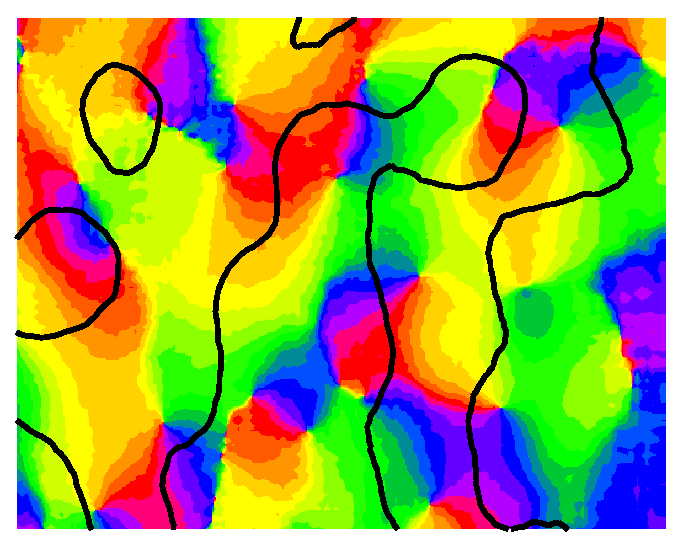
\epsfig{file=pics/odop_pict.eps,width=12.2cm}
\end{center}
\caption{Orientierungskarte aus A17 einer strabismischen Katze. "Uberlagert
dargestellt (schwarze Linien) sind die Grenzen zwischen den links-- und
rechts"augigen Dom"anen der im gleichen Experiment gemessenen
Okulardominanzkarte.}
\label{odop_pict}
\end{figure}

Anhand von Okulardominanz-- und Orientierungskarten aus A17 strabismischer
Katzen, die in Experimenten von Siegrid L"owel am Max--Planck--Institut
f"ur Hirnforschung gemessen wurden, konnte nun erstmals auch f"ur die Katze
eine solche Schnittwinkelstatistik erstellt werden. Bei strabismischen
Katzen ist der Grad der Okulardominanzsegregation sogar st"arker als im
Affen (vgl. Abschn.~\ref{unterschiede}, Abb.~\ref{okuhist}), und daher auch
die Okulardominanzkarte durch optisches Ableiten zug"anglich. Diese
experimentell gemessenen Karten liegen dabei als Bildmatrix vor (die im
Experiment verwendete CCD--Kamera liefert Bilder mit einer Aufl"osung von
$128\times 128$ Pixeln). Eine "Uberlagerung eines Ausschnittes des Bildes
der Orientierungskarte $\theta(\mathbf{x})$ mit dem Bild der Grenzlinien
der Okulardominanzkarte\footnote{F"ur jede Position $\mathbf{x}$ liegt ein
Wert zwischen $-1$ (linkes Auge) und $+1$ (rechtes Auge) vor. Die
Grenzlinie ist somit definiert als $o(\mathbf{x}) = 0$.} $o(\mathbf{x})$
zeigt Abb.~\ref{odop_pict}. Hier wird schon durch Augenschein wird
deutlich, da"s die Grenzen der Okulardominanzdom"anen die
Iso--Orientierungsgebiete h"aufig senkrecht schneiden.
\setcounter{footnote}{1}

Um diesen Zusammenhang zu quantifizieren, ben"otigt man die Schnittwinkel
zwischen den Iso--Orientierungslinien $\theta(\mathbf{x})=\theta_k$ und den
Okulardominanzgrenzlinien $o(\mathbf{x}) = 0$.  Die Richtung dieser
Konturen ist in jedem Punkt "uber Drehung der Feldgradienten bestimmbar;
"uber das Skalarprodukt dieser Gradienten erh"alt man die Schnittwinkel
$\alpha$ f"ur jeden Punkt $\mathbf{x}$ der Matrix:

\begin{equation*}
\alpha(\mathbf{x})=\text{acos}\!\left(\frac{\pmb\nabla\theta(\mathbf{x})
\;\pmb\nabla o(\mathbf{x})}{\vert\pmb\nabla\theta(\mathbf{x})\;\pmb\nabla
o(\mathbf{x})\vert}\right)
\end{equation*}

Zur Berechnung des r"aumlichen Gradienten $\pmb\nabla =
{\partial_1\choose\partial_2}$ auf dem Gitter wurde die diskrete
Approximation
\begin{equation*}
(\pmb\nabla\theta)_{ij}\approx\frac{1}{2\Delta}{{\theta_{i+1,j}\,-\,\theta_{i-1,j}}\choose{\theta_{i,j+1}\,-\,\theta_{i,j-1}}}
\end{equation*}
verwendet (analog f"ur $\pmb\nabla o$). Das Histogramm "uber die
resultierende Verteilung der Schnittwinkel auf den
Okulardominanzgrenzlinien $\alpha(\left\{\mathbf{x}^\prime\vert\;
o(\mathbf{x}^\prime)=0\right\})$ f"ur den Datensatz in Abb.~\ref{odop_pict}
zeigt Abb.~\ref{odop_hist}, Mitte. In allen vorliegenden Datens"atzen aus
insgesamt 7 untersuchten strabismischen Katzen wurde eine solche
$90^\circ$--Statistik der Schnittwinkelverteilung vorgefunden
\citeaffixed{loewel:1996}{siehe}.

Ein wichtiges Ph"anomen visueller Reizr"apresentationen sowohl bei Affen,
als auch wie hier gezeigt bei Katzen, ist demnach die lokale geometrische
Beziehung zwischen den Iso--Orientierungslinien und den Grenzen der
Okulardominanzdom"anen: Diese schneiden sich mit "uberwiegend stumpfen
Winkeln.

\begin{figure}[t]
\begin{center}
\epsfig{file=pics/odop_hist.eps,width=\textwidth}
\end{center}
\caption{Histogramme der Schnittwinkelverteilung zwischen den
Iso--Orien\-tier\-ungs\-linien und den Grenzlinien der Okulardominanzdom"anen
im ph"anomenologischen Modell (siehe Abschn.~\ref{modell}), der
strabismischen Katze \protect\citeaffixed{loewel:1996}{hier f"ur den in
Abb.~\ref{odop_pict} gezeigten Datensatz; weitere siehe} und den Affen
\protect\citeaffixed{oby:1993b}{Daten aus}.}
\label{odop_hist}
\end{figure}

\subsection{Entstehung neuronaler Karten durch Selbstorganisation}
\label{plastizitaet}

Die in den letzten Abschnitten skizzierte, besondere funktionale Anordnung
der Neurone im visuellen Cortex von Katzen und Affen wirft zwei
grundlegende Fragen auf \cite{marlsburg:1973}:

\begin{itemize}
\item Warum sind die Neurone so angeordnet?
\item Durch welche Mechanismen wird die Entstehung und Anordnung dieser
neuronalen Eigenschaften determiniert?
\end{itemize}

In der Diskussion um den Entstehungsmechanismus neuronaler Karten ist dabei
eine immer wiederkehrende Hypothese, da"s die diesen Karten
zugrundeliegende Verschaltung der Neurone genetisch prespezifiziert sein
k"onnte \citeaffixed{wiesel:1974,goedecke:1996}{vgl.}. Die Kodierung der
Struktur solcher Reizrepr"asentationen --- die nicht nur im visuellen
Cortex sondern auch in allen anderen Sinnessytemen angelegt sind --- im
Erbgut w"urde jedoch ein immenses Ma"s an genetischer Information
ben"otigen.  Ein weiteres Argument, das diese Hypothese unplausibel
erscheinen l"a"st, ist die Tatsache, da"s mit streng genetisch
determinierten Verschaltungen nicht der im Experiment beobachtete hohe Grad
der \emph{Plastizit"at} visueller Reizrepr"asentationen zu erkl"aren w"are.
 
Eine Vielzahl von Experimenten belegt jedoch eindrucksvoll, da"s die
Struktur --- zumindest aber die Feinstruktur --- visueller
Reizrepr"asentationen von der visuellen Erfahrung abh"angt. So f"uhrt
z.B. der Verschlu"s eines Auges in einem entwicklungsphysiologisch
kritischem Zeitraum nach der Geburt sowohl bei Katzen als auch bei Affen zu
einer deutlichen Abnahme des Anteils binokularer Neurone. Die mei"sten
Neurone antworten nach einem gewissen Zeitraum nur noch auf das ge"offnete
Auge \citeaffixed{shatz:1978,levay:1980}{siehe z.B.}. Auch die Struktur der
Orientierungskarte ist reizabh"angig; jedoch gibt es hierzu aufgrund der
schwierigeren Aufzucht der Tiere nicht dieselbe F"ulle an Experimenten wie
f"ur die Okulardominanz. \citeasnoun{blakemore:1970} zogen z.B. Katzen in
einer Umgebung auf, die nur aus horizontalen und vertikalen Reizen bestand:
Der Anteil der auf horizontal/vertikal spezialisierten Neurone
vergr"o"serte sich dadurch auf Kosten der sonstig orientierten Neurone.

Da"s die Anzahl der f"ur einen Sinnesreiz verantwortlichen Neurone mit der
H"aufigkeit des Autftretens des Reizes zusammenh"angt, ist dabei schon aus
anderen Sinnesbereichen bekannt.  So sind z.B. f"ur die tastsensiblen
Fingerkuppen mehr Neurone verantwortlich als f"ur einen vergleichbar
gro"sen Ausschnitt des Ellenbogenbereichs. Die zahlreichen
Deprivationsexperimente am visuellen System von Katzen und Affen zeigen
deutlich, da"s diese Anzahl in einem dynamischen Proze"s an eine
ver"anderte Reizumgebung angepa"st werden kann.

Die Basis f"ur diese Adaptionsf"ahigkeit des Gehirns ist dabei nach
heutigem Kenntnistand die Variabilit"at der Verbindungsst"arken zwischen
den Neuronen.  Die Ver"anderung der Verbindungsst"arken findet vorwiegend
an \emph{Synapsen}, den ``Kontaktstellen'' zwischen den Neuronen statt.
Nach einer auf \citeasnoun{hebb:1949} zur"uckgehenden Vorstellung "andert
sich die Wirksamkeit einer Synapse in Abh"angigkeit von der Korrelation
zwischen den Aktivit"aten des \emph{pr"asynaptischen}, d.h. des die Synapse
ansteuernden, und des \emph{postsynaptischen}, d.h. des von der Synapse
angesteuerten Neurons. Diese Vorstellung konnte an einzelnen Synapsen auch
experimentell nachgewiesen werden \cite{brown:1990,kirkwood:1994}.  Die
Hebb'sche Lernregel erm"oglicht die Ausrichtung der Architektur des
Nervensystems an die Struktur der Umwelt, wobei wichtige, d.h. h"aufig
vorkommende Ereignisse, st"arker ber"ucksichtigt werden als unwichtige
(seltene). Anhand dieser Lernregel kann das Hirn un"uberwacht signifikante
Merkmale aus der Umwelt extrahieren.

Eine viel plausiblere Hypothese f"ur die Entstehung visueller
Reizrepr"asentationen ist daher, da"s diese ihre Struktur spontan durch
einen Proze"s aktivit"atsabh"angiger Selbstorganisation ausbilden.  Zum
einen bedarf die Kodierung von Selbstorganisationsregeln im Erbgut --- die
leicht abgewandelt vielleicht auch in anderen Sinnessystemem zur Geltung
kommen k"onnten --- eines viel geringeren Ma"ses an genetischer
Information.  Viel wesentlicher ist aber, da"s die aktivit"atsabh"angige
Selbstorganisation einen geeigneten Mechanismus zur Erkl"arung der
beobachteten Plastizit"at der Reizrepr"asentationen darstellt.
